%%%%%%%%%%%%%%%%%%%%%%%%%%%%%%%%%%%%%%%%%%%%%%%%%%%%%%%%%%%%%%%%%%%%%%%%%%%%%%%%%%%%%%%%%%
%%
%% Description:		This is an example presentation using the beamerthemedhbw
%%
%%					The beamerthemedhbw is based on jacksbeamertheme
%%					(https://github.com/JacknJo/jacksbeamertheme)
%%
%% Author:			Hannes Bartle																				
%% 					DHBW Ravensburg Campus Friedrichshafen		
%%					September 2016	
%% 
%% The beamerthemedhbw is free software: you can redistribute it and/or modify
%% it under the terms of the GNU General Public License as published by
%% the Free Software Foundation, either version 3 of the License, or
%% (at your option) any later version.
%% 
%% The beamerthemedhbw is distributed in the hope that it will be useful,
%% but WITHOUT ANY WARRANTY; without even the implied warranty of
%% MERCHANTABILITY or FITNESS FOR A PARTICULAR PURPOSE.  See the
%% GNU General Public License for more details.
%% 
%% You should have received a copy of the GNU General Public License
%% along with the beamerthemedhbw.  If not, see <http://www.gnu.org/licenses/>.
%% 
%% 
%%%%%%%%%%%%%%%%%%%%%%%%%%%%%%%%%%%%%%%%%%%%%%%%%%%%%%%%%%%%%%%%%%%%%%%%%%%%%%%%%%%%%%%%%%


\documentclass[	12pt, 				
				t,					
				aspectratio=169,
				%handout
				]{beamer}


\usepackage[utf8]{inputenc}
\usepackage[english, ngerman]{babel}
\usepackage[T1]{fontenc}
\usepackage{tikz}
\usepackage{ifthen}
\usepackage{xcolor}
\usepackage{makecell}
\usetikzlibrary{shadows.blur}

\newlength{\forkmeoffset}
\setlength{\forkmeoffset}{12em}
\definecolor{forkmebg}{HTML}{CC0000}
\definecolor{forkmefg}{HTML}{EEEEEE}

\newcommand{\forkme}[1][west]{
	\ifthenelse{\equal{#1}{east}}{%
		\tikzset{forkmerot/.style={rotate=-45}}
	}{%
		\tikzset{forkmerot/.style={rotate=45}}
	}
	\begin{tikzpicture}[remember picture, overlay]
	\node[forkmerot, shift={(0, -\forkmeoffset)}] at (current page.north #1) {
		\begin{tikzpicture}[remember picture, overlay]
		\node[fill=forkmebg, text centered, minimum width=50em, minimum height=3.0em, blur shadow, shadow yshift=0pt, shadow xshift=0pt, shadow blur radius=.4em, shadow opacity=50, text=forkmefg](fmogh) at (0pt, 0pt) {   \fontfamily{phv}\selectfont\bfseries Fork me on GitHub};
		\draw[forkmefg!60, dashed, line width=.08em, dash pattern=on .5em off 1.5\pgflinewidth] (-25em,1.2em) rectangle (25em,-1.2em);
		\end{tikzpicture}
	};
	\end{tikzpicture}
}

\title{Programmieren II}
\date{Ravensburg\\\today}
\author{Lukas Abelt \\\texttt{lukas.abelt@airbus.com}}
\institute{DHBW Ravensburg \\ Wirtschaftsinformatik}

\usetheme{dhbw}
\renewcommand{\usecompanylogo}{1}

\newcommand{\printcompanylogo}{
\includegraphics[width=4cm]{graph/airbus_logo.png}}

\newcommand{\middleText}{Lukas Abelt}
\newcommand{\outlineSection}{Inhalt}

\setlength{\framesubtitleoffset}{0pt}
\setlength{\frametitleoffset}{0.05cm}
\setlength{\frametextoffset}{0.1cm}
\setlength{\framefootlineoffset}{0cm}


\begin{document}
	
	\begin{frame}[noframenumbering]
		\titlepage
	\end{frame}


	\begin{frame}{Outline}
		\tableofcontents
	\end{frame}

	\outlineFrame{Über mich}
	
	\begin{frame}{Allgemeines}{Wer bin ich?}
		\begin{itemize}
			\item Lukas Abelt
			\item <2-> 21 Jahre (Jahrgang '97)
			\item <3-> Ursprünglich aus Werder (Havel)
			\begin{itemize}
				\item <4->...in Brandenburg
				\item <5->...bei Potsdam
				\begin{itemize}
					\item <6->...bei Berlin
				\end{itemize}
			\end{itemize}
		\end{itemize}
	\end{frame}
	
	\begin{frame}{Allgemeines}{Wo komme ich her?}
		\begin{minipage}{0.7\textwidth}
		\centering
			\begin{figure}
			\centering
			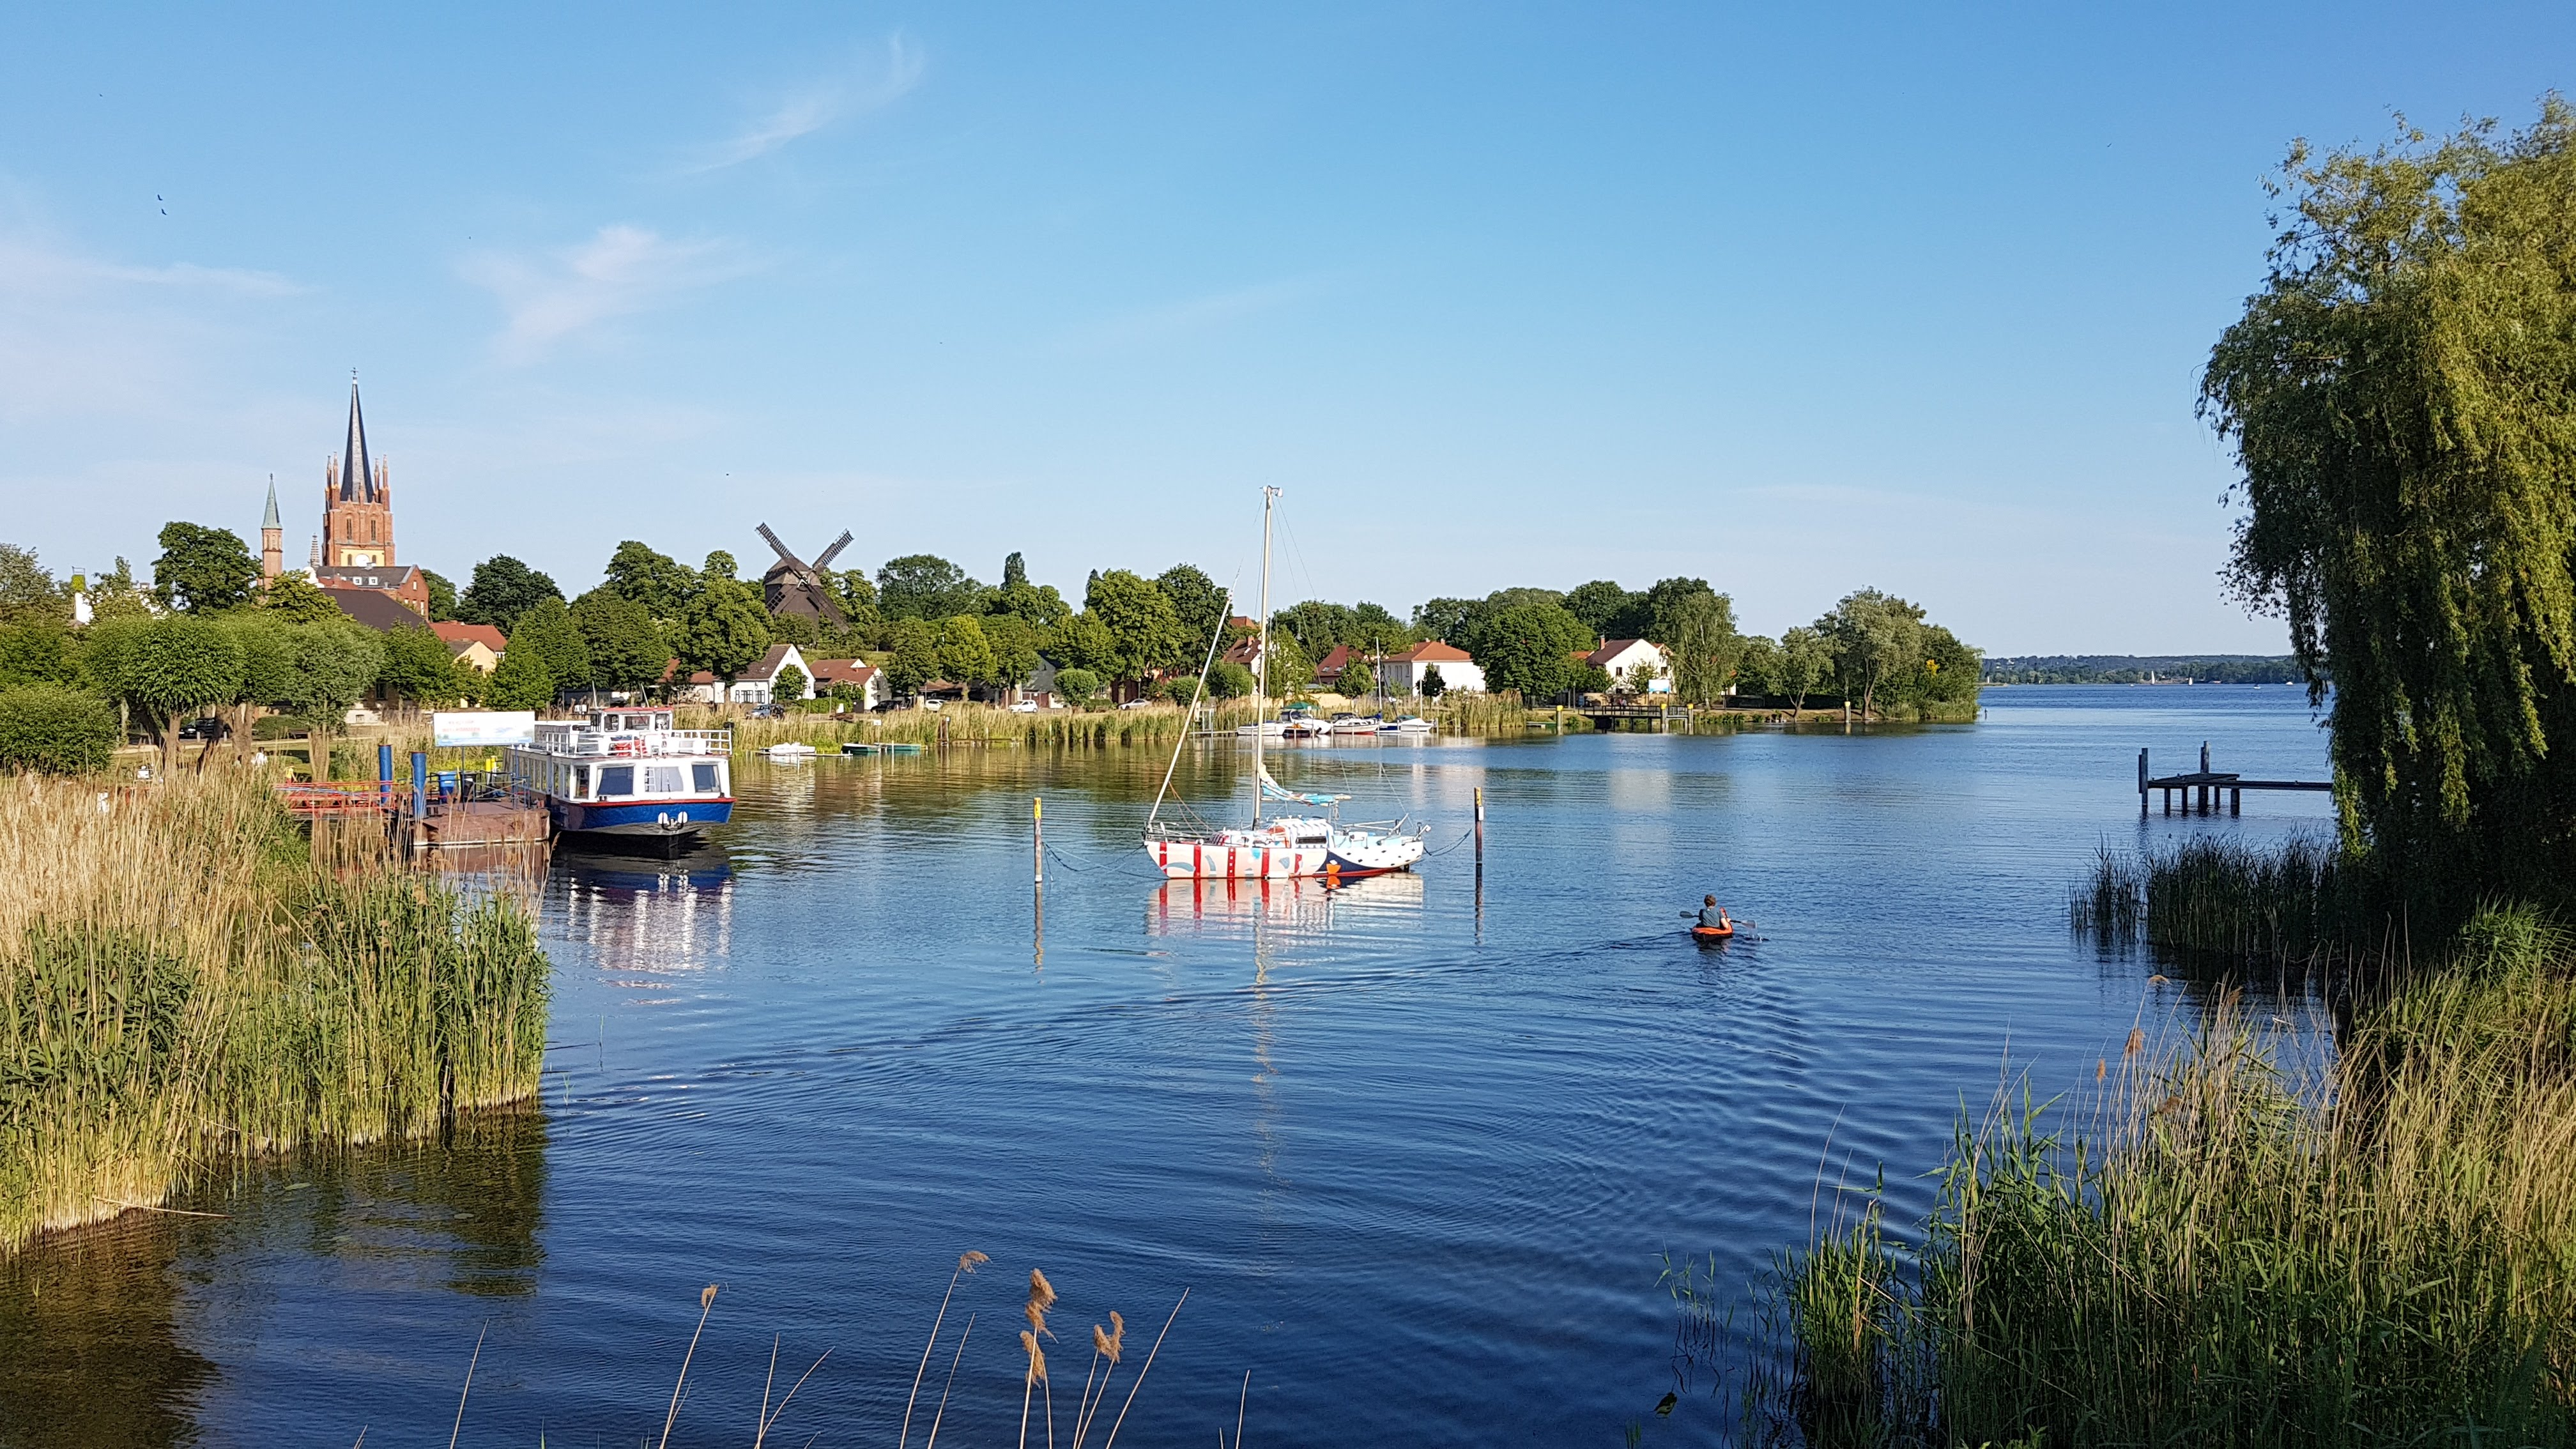
\includegraphics[width=.95\linewidth]{graph/werder.jpg}
		\end{figure}
		\end{minipage}%
		\begin{minipage}{0.3\textwidth}
		\centering
			\begin{figure}
			\centering
			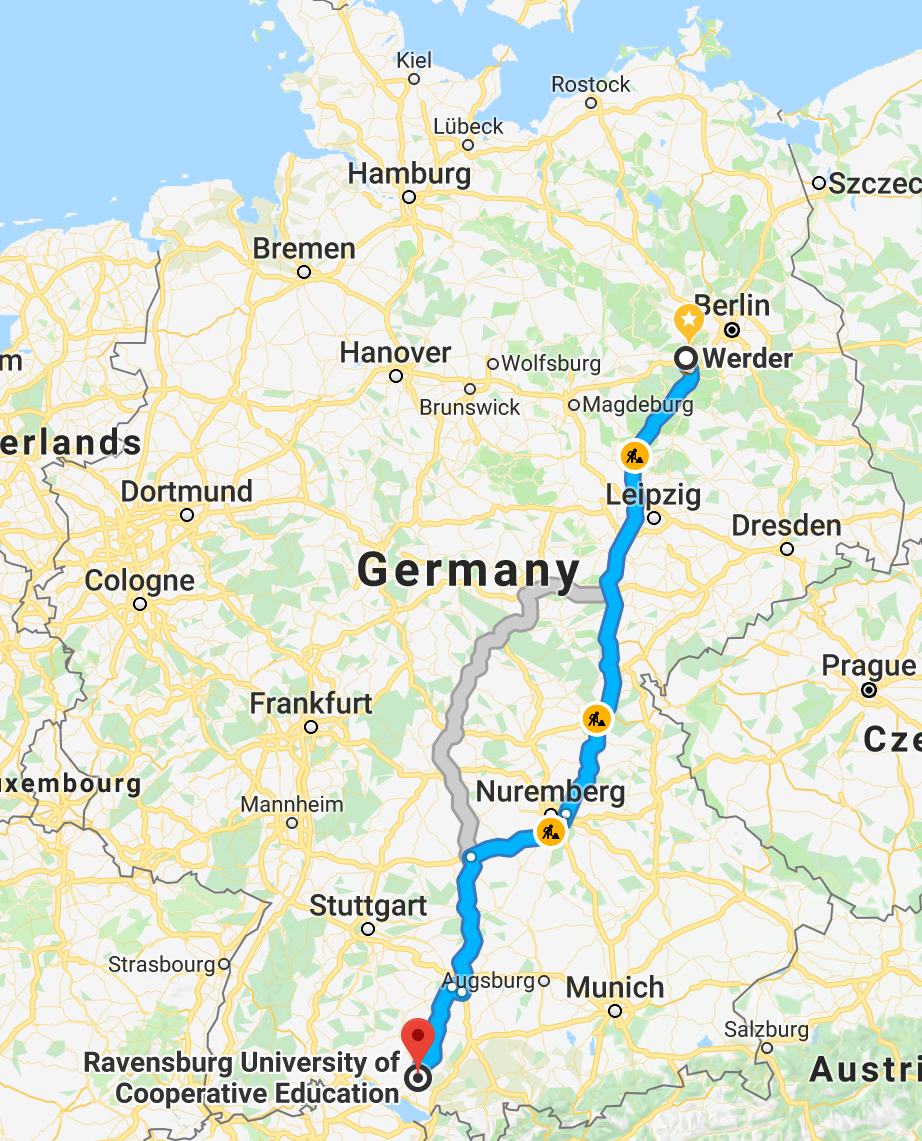
\includegraphics[width=.95\linewidth]{graph/route2werder.png}
			\end{figure}
		\end{minipage}
		\\
		\tiny{Bildquelle: \url{https://upload.wikimedia.org/wikipedia/commons/4/47/Werder_an_der_Havel.jpg} (Abgerufen: 26.02.2019)}
	\end{frame}

	\begin{frame}{Beruflicher\&Akademischer Werdegang}{}
		\begin{itemize}
			\item \textbf{Juli 2015} - Abitur
			\item \textbf{Ab September 2015} - Duales Studium
			\begin{itemize}
				\item Hochschule: DHBW Ravensburg \textbf{Campus Friedrichshafen}
				\item Studiengang: Informationstechnik (Mobile Informatik)
				\item Firma: Airbus Defence and Space (Immenstaad)
			\end{itemize}
			\item \textbf{September 2018} - Bachelorarbeit und -abschluss
			\item \textbf{Seit Oktober 2018} - Software Architect bei Airbus
		\end{itemize}
	\end{frame}
	
	\begin{frame}{Was habe ich bisher gemacht?}{Praxisphasen}
			\begin{itemize}
				\item Arbeit im Bereich SIGINT(Signal Intelligence)
				\item Implementierung des TCP Stacks zur Übertragung von Signaldaten(C++, Matlab, Simulink)
				\item Später Abteilungswechsel zu Simulationssoftware
				\item Implementierung eines neuen Schadenmodells in das bestehende System (C++)
				\item \textbf{Analyse und Bewertung neuer Methoden zur Durchführung simulationsgestützter Parameterstudien mit cloud-basierten Systemen} (Bachelorarbeitsthema)
			\end{itemize}
	\end{frame}
	
	\begin{frame}{Was habe ich bisher gemacht?}{Theoriephasen}
		\begin{itemize}
			\item Mathetutorium für Semester 1
			\item Mathetutorium für Semester 2
			\item Studienarbeit: Entwickeln eines selbstlernenden Chatbots (Tensorflow, Python)
			\begin{itemize}
				\item Erfolgreiche Zielerreichung fraglich?
			\end{itemize}
			\item 3. Platz beim Bierathlon 2016
			\item Organisator des alljährlichen Glühweingrillens Friedrichshafen (Nächster Termin: April 2019)
		\end{itemize}
	\end{frame}
	
	\begin{frame}{Was habe ich bisher gemacht?}{Studienarbeit}
		"`they're just fucking fucking fucking not just fucking with"'
	\end{frame}
	
	\outlineFrame{Vorlesung}
	
	
	% Allgemeines
	%	Script x
	%	Organisation x
	
	% Ziele x
	%	Laut Modulbeschreibung x
	%	Mein Ziel x
	
	% Themen & Termine x
	
	% Prüfungsleistung

\begin{frame}{Allgemeines}{Skript}
	\begin{itemize}
		\item Mit \LaTeX{} erstellt
		\item Im Druck verfügbar...
		\begin{itemize}
			\item ...wenn man bezahlt hat
		\end{itemize}
		\item Digitale Version als PDF verfügbar
		\item Source Code zum selbst compilen auf GitHub verfügbar:
		\begin{itemize}
			\item \small{\url{https://github.com/LuAbelt/WI18\_ProgrammierenII}}
		\end{itemize}
	\end{itemize}
	\begin{block}{Git repository clonen}
		\tt{git clone https://github.com/LuAbelt/WI18\_ProgrammierenII}
	\end{block}
\end{frame}

\begin{frame}{Allgemeines}{Skript}
	{\small \setlength{\forkmeoffset}{2.5cm} \forkme[east]}
	\begin{minipage}{\textwidth}
		\centering	
		
\includegraphics[height=0.6\textheight]{graph/gitqr.png}
	\end{minipage}
\end{frame}

\begin{frame}{Allgemeines}{Organisation}
	\begin{itemize}
		\item Insgesamt 60 UE über 15 Termine
		\item Also 4 UE pro Termin
		\item Aufteilung (Vorschlag)
		\begin{itemize}
			\item 2 UE Theorie
			\item Kaffeepause
			\item 2 UE praktische Anwendung
		\end{itemize}
	\end{itemize}
\end{frame}
\begin{frame}{Allgemeines}{Organisation}
	\begin{itemize}
		\item Zu (fast) jedem Termin wird es eine praktische Aufgabe zur Implementierung geben (Für den zweiten Vorlesungsteil)
		\item Aufgaben \& meine Beispielimplementierung: Nach der Vorlesung im Git Repo zu finden
		\item Beispielimplementierung wird immer in Java sein
		\item Hinweise:
		\begin{itemize}
			\item Ich empfehle IntelliJ als IDE (Für Studenten kostenlose Pro Version)
			\item DHBW Rechner haben (leider) nur Eclipse
			\item Im Git wird es Projektdateien für bei IDE's geben
		\end{itemize}
	\end{itemize}
\end{frame}

\begin{frame}{Allgemeines}{Feedback}
	\begin{itemize}
		\item Auch ich bin nicht unfehlbar
		\begin{itemize}
			\item Hauptsächlich in C++ unterwegs
			\item Dadurch ggf. Ungenauigkeiten und Fehler bei Java spezifischen Aspekten
		\end{itemize}
		\item Fragen gerne immer und sofort
		\item ...Gleiches gilt für (themenbezogene) Diskussionen
		\item Feedback gerne über alle Kanäle wie zum Beispiel:
		\begin{itemize}
			\item Persönlich
			\item Per Mail
			\item Über GitHub/GitLab
			\item usw...
		\end{itemize}
		\item Kontakdaten am Ende jedes Foliensatzes
	\end{itemize}
\end{frame}

\begin{frame}{Ziele der Vorlesung I}{Laut Modulbeschreibung}
	\vfill
	\begin{block}{Fachkompetenz}
		Die Studierenden kennen fortgeschrittene Konzepte objektorintierter Programmiersprachen. Sie besitzen Kenntnisse über wichtige Algorithmen und Datenstrukturen sowie Methoden
		zur Beurteilung der Effizienz und Qualität von Algorithmen.
	\end{block}
	\vfill
\end{frame}

\begin{frame}{Ziele der Vorlesung II}{Laut Modulbeschreibung}
	\vfill
	\begin{block}{Methodenkompetenz}
		Die Studierenden können fortgeschrittene Konzepte der Objektorientierung anwenden und autonom mittlere bis größere lauffähige Programme implementieren und testen. Sie sind in der Lage, Algorithmen verschiedener Darstellungsarten zu 
		verstehen und ihre Effizienz bzw. Qualität zu beurteilen, aber auch selbstständig Algorithmen und dazu erforderliche Datenstrukturen zu entwickeln und zu implementieren.
	\end{block}
	\vfill
\end{frame}

\begin{frame}{Ziele der Vorlesung III}{Laut Modulbeschreibung}	
	\vfill
	\begin{block}{Personale und Soziale Kompetenz}
		Die Studierenden können eigenständig Algorithmen und Lösungsverfahren erarbeiten. Sie können stichhaltig und sachangemessen über Konzepte und eigene Algorithmen und deren Implementierung 
		und die damit verbundenen Probleme argumentieren, eigene Umsetzungen plausibel darstellen und eventuelle Fehler nachvollziehbar gegenüber anderen begründen.
	\end{block}
	\vfill
\end{frame}
	
\begin{frame}{Ziele der Vorlesung IV}{Laut Modulbeschreibung}
	\vfill
	\begin{block}{Übergreifende Handlungskompetenz}
		Die Studierenden können unter Einsatz der Programmiersprache komplexe praktische Probleme modellieren, algorithmisch behandeln und in anwenderfreundliche und effiziente Lösungen umsetzen. Sie 
		können praktische Problemstellungen analysieren und bekannte Algorithmen und Datenstrukturen effizienzorientiert darauf anwenden und falls notwendig an die Problemstellung anpassen.
	\end{block}
	\vfill
\end{frame}

\begin{frame}{Ziele der Vorlesung V}{In meinen Worten}
	\vfill
	\begin{alertblock}{Kurzgesagt}
		Am Ende der Vorlesung sollt ihr mit den vorgestellten Konzepten der fortgeschrittenen Objektorientierung vertraut sein. Dies beinhaltet unter anderem das theoretische Verständnis der zugrundeliegenden Konzepte,
		sowie die \textbf{sprachunabhängige} Anwendung des gelernten. Ziel ist \textbf{nicht} das lernen von Java, sondern das übergreifende Verständnis, sodass das gelernte (theoretisch) in jeder Sprache angewandt werden kann!
	\end{alertblock}
	\vfill
\end{frame}

\begin{frame}{Termine \& Themen}
	\begin{itemize}
		\item \textbf{01.04.2019, 14:00-17:15}:
		\begin{itemize}
			\item Vorstellung
			\item Allgemeine Informationen zur Vorlesung
			\item Datentypen
		\end{itemize}
		\item \textbf{03.04.2019, 14:00-17:15}:
		\begin{itemize}
			\item Generische Interfaces \& Klassen
			\item Nutzung der Klassenbibliothek
		\end{itemize}
		\item \textbf{08.04.2019, 14:00-17:15}:
		\begin{itemize}
			\item Algorithmen Teil 1
			\begin{itemize}
				\item Beschreibung
				\item Analyse
			\end{itemize}
		\end{itemize}
	\end{itemize}
\end{frame}

\begin{frame}{Termine \& Themen}
	\begin{itemize}
		\item \textbf{10.04.2019, 14:00-17:15}:
		\begin{itemize}
			\item Listenstrukturen Teil 1
			\begin{itemize}
				\item Grundoperationen
				\item Arrays
				\item Verkettete Listen
			\end{itemize}
		\end{itemize}
		\item \textbf{24.04.2019, 14:00-17:15}:
		\begin{itemize}
			\item Listenstrukturen Teil 2
			\begin{itemize}
				\item Stacks
				\item Queues
				\item Bäume
			\end{itemize}
		\end{itemize}
	\end{itemize}
\end{frame}

\begin{frame}{Termine \& Themen}
	\begin{itemize}
		\item \textbf{25.04.2019, 14:00-17:15}:
		\begin{itemize}
			\item Abstrakte Datentypen
			\begin{itemize}
				\item Collections
				\item Iteratoren
			\end{itemize}
		\end{itemize}
		\item \textbf{29.04.2019, 14:00-17:15}:
		\begin{itemize}
			\item Algorithmen Teil 2
			\begin{itemize}
				\item Suchverfahren
			\end{itemize}
		\end{itemize}
		\item \textbf{02.05.2019, 14:00-17:15}:
		\begin{itemize}
			\item Algorithmen Teil 3
			\begin{itemize}
				\item Sortierverfahren
			\end{itemize}
		\end{itemize}
	\end{itemize}
\end{frame}

\begin{frame}{Termine \& Themen}
	\begin{itemize}
		\item \textbf{06.05.2019, 14:00-17:15}:
		\begin{itemize}
			\item Algorithmen Teil 4
			\begin{itemize}
				\item Divide\&Conquer
				\item Backtracking
			\end{itemize}
		\end{itemize}
		\item \textbf{08.05.2019, 14:00-17:15}:
		\begin{itemize}
			\item Fortgeschrittene Konzepte Teil 1
			\begin{itemize}
				\item Parallelisierung
				\item Synchronisationskonzepte
			\end{itemize}
		\end{itemize}
		\item \textbf{13.05.2019, 14:00-17:15}:
		\begin{itemize}
			\item Fortgeschrittene Konzepte Teil 2
			\begin{itemize}
				\item Synchronisationskonzepte
				\item Ein- und Ausgabe über Streams
			\end{itemize}
		\end{itemize}
	\end{itemize}
\end{frame}

\begin{frame}{Termine \& Themen}
	\begin{itemize}
		\item \textbf{15.05.2019, 14:00-17:15}:
		\begin{itemize}
			\item Aufbau grafischer Oberflächen Teil 1
			\begin{itemize}
				\item Layout
				\item Typische Komponenten
			\end{itemize}
		\end{itemize}
		\item \textbf{20.05.2019, 14:00-17:15}:
		\begin{itemize}
			\item Aufbau grafischer Oberflächen Teil 2
			\begin{itemize}
				\item Typische Komponenten
				\item Ereignisbehandlung
			\end{itemize}
		\end{itemize}
		\item \textbf{22.05.2019 \& 27.05.2019}:
		\begin{itemize}
			\item Puffertermin
		\end{itemize}
	\end{itemize}
\end{frame}

\begin{frame}{Puffertermine}{}
	\begin{itemize}
		\item Geplante Themen sind nach vorraussichtlich 13 Terminen abgearbeitet
		\item Sofern es nicht zu Verzögerungen kommt, könnte man diese nutzen für:
		\begin{itemize}
			\item Wiederholungen
			\item Exkurse zu anderen Themen der SW-Entwicklung
			\item Freies arbeiten für die Prüfungsleistung
		\end{itemize}
		\item Gestaltung der Puffertermine frei nach euren Interessen
	\end{itemize}
\end{frame}

\begin{frame}{Prüfungsleistung}{}
	\begin{itemize}
	\item \textbf{Keine} Klausur, denn:
		\begin{itemize}
			\item Schon 6 Klausuren dieses Semester
			\item Rein theoretische Überprüfungen für Programmieren sowieso eher fraglich
		\end{itemize}
	\item Stattdessen: \textbf{Portfolioprüfung}
		\begin{itemize}
			\item Besteht aus mehreren Teilleistungen (Hier: 3)
			\item Teil 1: Kurztest
			\item Teil 2\&3: Programmentwurf inklusive Dokumentation 
		\end{itemize}
	\end{itemize}
\end{frame}

\begin{frame}{Prüfungsleistung}{Kurztest}
	\textbf{Teil 1: Kurztest}
	\begin{itemize}
		\item Zu Themenblöcken Algorithmen und Datentypen
		\item Bearbeitungszeit: ~30 Minuten
		\item Noch kein fester Termin gesetzt
		\item Gewichtung an der Gesamtnote: \textbf{20\%}
	\end{itemize}
\end{frame}

\begin{frame}{Prüfungsleistung}{Programmentwurf}
	\textbf{Teil 2: Programmentwurf}
	\begin{itemize}
		\item Wird Teilaspekte aus (fast) allen Themenblöcken enthalten
		\begin{itemize}
			\item Vermutlich Schwerpunkt auf Datenstrukturen
			\item Vermutlich keine (oder wenig) Teile aus grafischen Overflächen
		\end{itemize}
		\item Zu bearbeiten in Gruppen von 3-4 Personen
		\item Bearbeitungszeit: ~4 Wochen
		\item Umsetzung empfohlen in Java
		\begin{itemize}
			\item Jedoch nicht darauf beschränkt!
			\item Bei Interesse Details bei mir erfragen
		\end{itemize}
		\item Gewichtung an der Gesamtnote: \textbf{50\%}
	\end{itemize}
\end{frame}

\begin{frame}{Prüfungsleistung}{Dokumentation}
	\textbf{Teil 3: Dokumentation}
	\begin{itemize}
		\item Dokumentation der im Programmentwurf implementierten Lösung
		\item Bearbeitungszeit: 4 Wochen (Parallel zum Programmentwurf)
		\item Gleiche Gruppen wie im Programmentwurf
		\item Gewichtung an der Gesamtnote: \textbf{30\%}
	\end{itemize}
\end{frame}
	
	\section*{Kontakt}
	\begin{frame}{Kontakt}{}
	\begin{itemize}
		\item E-Mail: \href{mailto:lukas.abelt@airbus.com}{lukas.abelt@airbus.com}
		\item GitHub: \url{https://www.github.com/LuAbelt}
		\item GitLab: \url{https://www.gitlab.com/LuAbelt}
		\item Telefon(Firma): 07545 - 8 8895
		\item Telegram: LuAbelt
	\end{itemize}
\end{frame}
	

\end{document}